% Options for packages loaded elsewhere
\PassOptionsToPackage{unicode}{hyperref}
\PassOptionsToPackage{hyphens}{url}
%
\documentclass[
  12pt,
]{article}
\usepackage{amsmath,amssymb}
\usepackage{iftex}
\ifPDFTeX
  \usepackage[T1]{fontenc}
  \usepackage[utf8]{inputenc}
  \usepackage{textcomp} % provide euro and other symbols
\else % if luatex or xetex
  \usepackage{unicode-math} % this also loads fontspec
  \defaultfontfeatures{Scale=MatchLowercase}
  \defaultfontfeatures[\rmfamily]{Ligatures=TeX,Scale=1}
\fi
\usepackage{lmodern}
\ifPDFTeX\else
  % xetex/luatex font selection
    \setmainfont[]{Times New Roman}
\fi
% Use upquote if available, for straight quotes in verbatim environments
\IfFileExists{upquote.sty}{\usepackage{upquote}}{}
\IfFileExists{microtype.sty}{% use microtype if available
  \usepackage[]{microtype}
  \UseMicrotypeSet[protrusion]{basicmath} % disable protrusion for tt fonts
}{}
\makeatletter
\@ifundefined{KOMAClassName}{% if non-KOMA class
  \IfFileExists{parskip.sty}{%
    \usepackage{parskip}
  }{% else
    \setlength{\parindent}{0pt}
    \setlength{\parskip}{6pt plus 2pt minus 1pt}}
}{% if KOMA class
  \KOMAoptions{parskip=half}}
\makeatother
\usepackage{xcolor}
\usepackage[margin=1in]{geometry}
\usepackage{graphicx}
\makeatletter
\def\maxwidth{\ifdim\Gin@nat@width>\linewidth\linewidth\else\Gin@nat@width\fi}
\def\maxheight{\ifdim\Gin@nat@height>\textheight\textheight\else\Gin@nat@height\fi}
\makeatother
% Scale images if necessary, so that they will not overflow the page
% margins by default, and it is still possible to overwrite the defaults
% using explicit options in \includegraphics[width, height, ...]{}
\setkeys{Gin}{width=\maxwidth,height=\maxheight,keepaspectratio}
% Set default figure placement to htbp
\makeatletter
\def\fps@figure{htbp}
\makeatother
\setlength{\emergencystretch}{3em} % prevent overfull lines
\providecommand{\tightlist}{%
  \setlength{\itemsep}{0pt}\setlength{\parskip}{0pt}}
\setcounter{secnumdepth}{5}
% preamble.tex
\usepackage{setspace}
\setstretch{1} % ensures single spacing

\usepackage{titlesec}
\titleformat{\section}{\normalfont\bfseries\Large}{\thesection}{1em}{}
\titlespacing\section{0pt}{12pt plus 4pt minus 2pt}{8pt plus 2pt minus 2pt}

\titleformat{\subsection}{\normalfont\bfseries\large}{\thesubsection}{1em}{}
\titlespacing\subsection{0pt}{10pt plus 2pt minus 2pt}{6pt plus 1pt minus 1pt}
\usepackage{float}
\usepackage[sorting=none]{biblatex}
\ifLuaTeX
  \usepackage{selnolig}  % disable illegal ligatures
\fi
\usepackage[]{biblatex}
\addbibresource{references.bib}
\usepackage{bookmark}
\IfFileExists{xurl.sty}{\usepackage{xurl}}{} % add URL line breaks if available
\urlstyle{same}
\hypersetup{
  pdftitle={Crop Production and Economic Impact in the U.S.},
  pdfauthor={Batsambuu Batbold},
  hidelinks,
  pdfcreator={LaTeX via pandoc}}

\title{Crop Production and Economic Impact in the U.S.}
\usepackage{etoolbox}
\makeatletter
\providecommand{\subtitle}[1]{% add subtitle to \maketitle
  \apptocmd{\@title}{\par {\large #1 \par}}{}{}
}
\makeatother
\subtitle{STAT 155 · Macalester College · Spring 2025}
\author{Batsambuu Batbold}
\date{}

\begin{document}
\maketitle

\section{Introduction}\label{introduction}

According to the Economic Research Service at the U.S. Department of
Agriculture, the top five U.S. crop cash receipts in 2023 were corn,
soybeans, fruits and nuts, vegetables and melons, and wheat
\cite{usda2023crops}.

\begin{figure}[H]
    \centering
    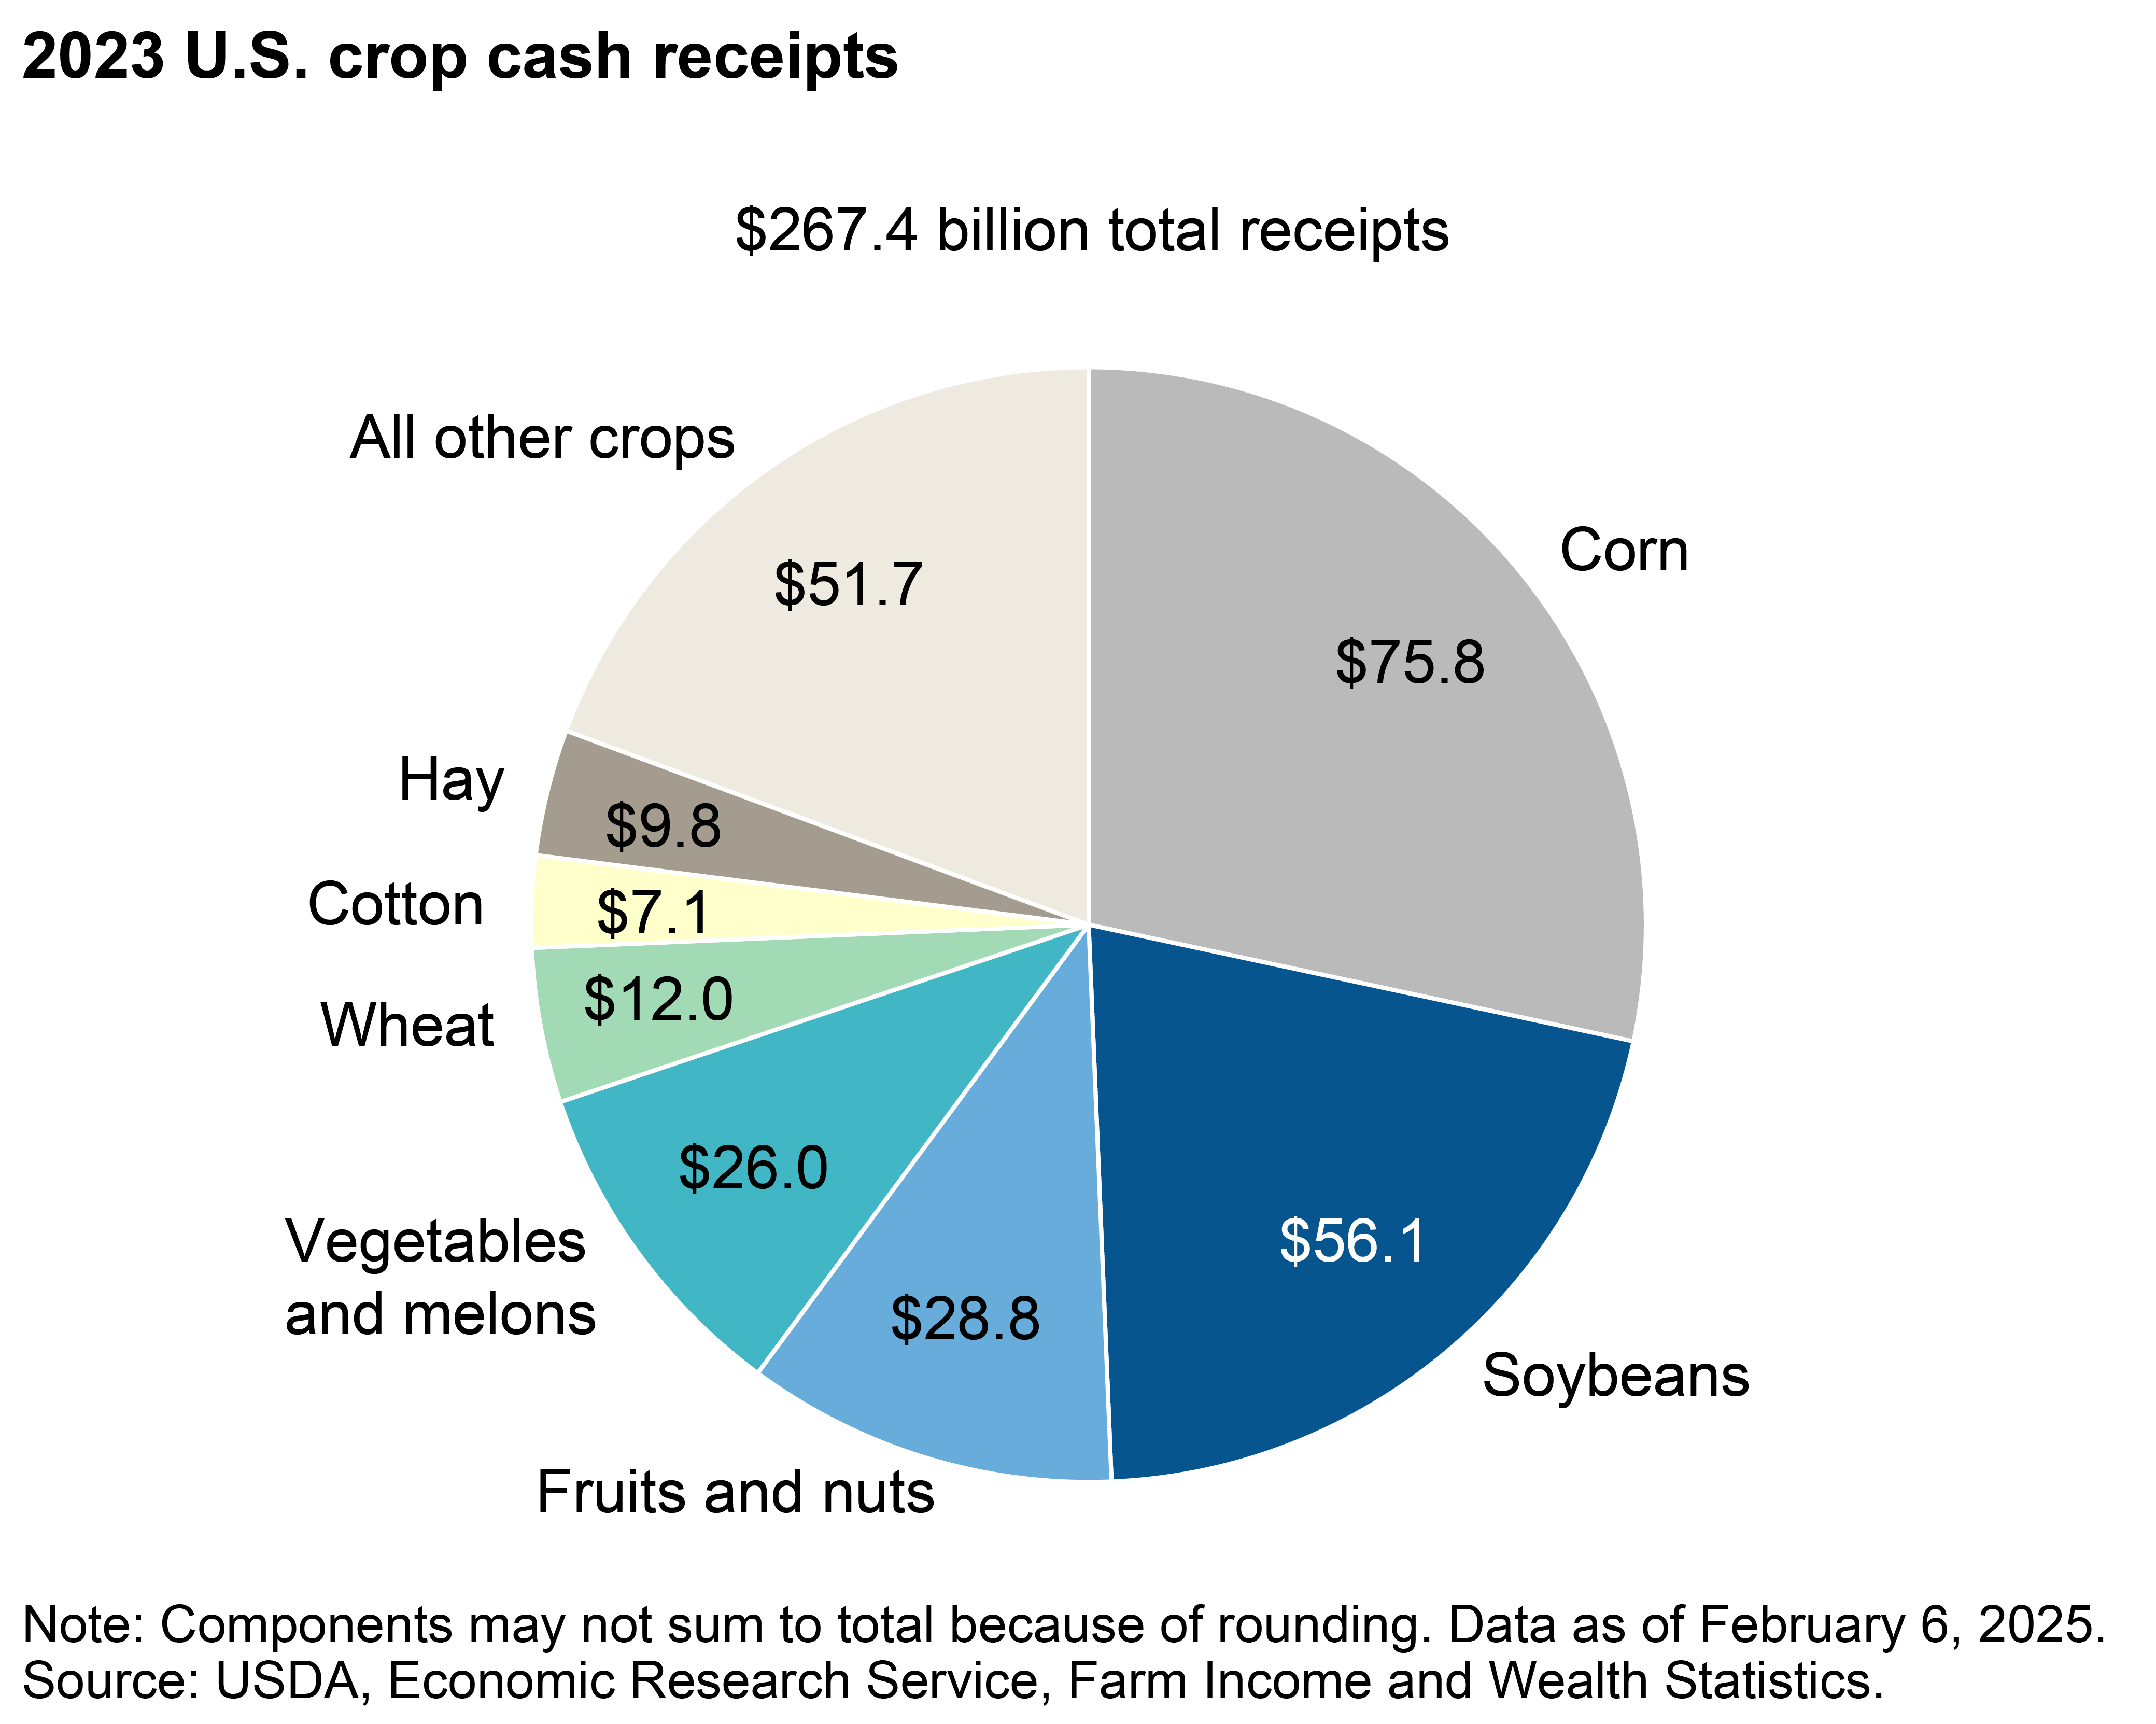
\includegraphics[width=0.6\textwidth]{2023cropcash.png}
    \caption{Image source: USDA ERS}
\end{figure}

To further understand how these cash crops contribute to the overall
economy, we are interested in the relationship between crop production
and GDP. Thus, our research question is:

\vspace{0.5em}

\begin{center}
\textbf{\textit{Is higher production of major cash crops (corn, soybeans, and wheat) significantly associated with higher county-level GDP?}}
\end{center}

\vspace{0.5em}

Understanding how agricultural productivity connects to economic
performance can help inform resource allocation in rural economies and
guide agricultural policy at both the state and federal levels.

\section{Data and Exploratory Data
Analysis}\label{data-and-exploratory-data-analysis}

Our datasets come from the U.S. Department of Agriculture (USDA)
\cite{usda} for crop data, and the Bureau of Economic Analysis (BEA)
\cite{bea} for GDP data. They cover all U.S. counties reporting 2022
agricultural data for at least one of the three major crops - corn,
soybeans, or wheat - along with corresponding GDP figures. Since the
most recent complete dataset on crop production is from 2022, we focus
our analysis on that year.

Because we are interested in the economic implications of agricultural
productivity, our outcome variable is county GDP (measured in thousands
of chained 2017 U.S. dollars), as it reflects overall economic
performance. Our predictors, based on available data, include:

\begin{itemize}
\tightlist
\item
  Production (in bushels),
\item
  Area harvested (in acres),
\item
  Sales (in U.S. dollars), and
\item
  Crop type (corn, soybeans, or wheat).
\end{itemize}

During our exploratory analysis, we found a clear positive association
between sales and production (Figure 2). Among the three crops, corn
requires the most production to generate a given amount of sales, while
soybeans require the least, reflecting their relative market prices.

\begin{figure}[H]
    \centering
    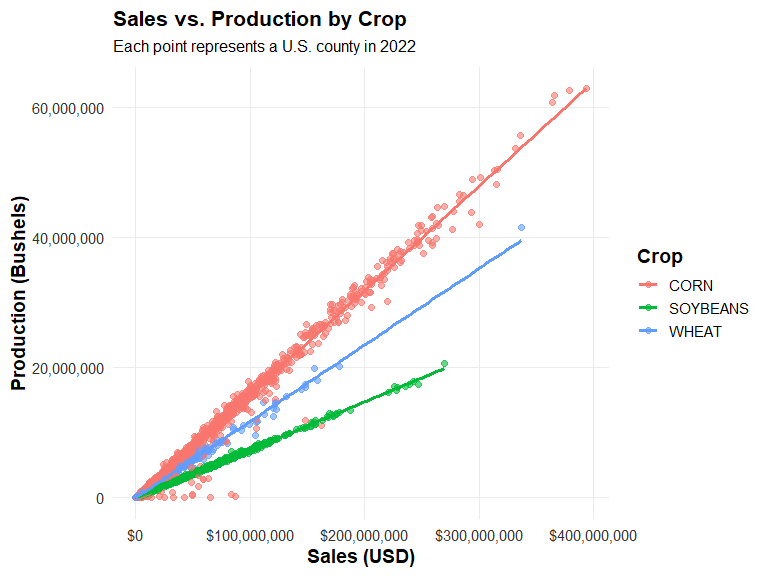
\includegraphics[width=0.9\textwidth]{prod_sale.png}
    \caption{Sales vs. Production by Crop. Each point represents a county-crop observation. Soybeans yield higher sales per bushel compared to corn and wheat, suggesting price differences.}
\end{figure}

We also observed that higher harvested area is associated with higher
production across all crops (Figure 3). Among them, corn appears the
most area-efficient, while wheat requires the most acreage to produce
the same quantity of output.

\begin{figure}[H]
    \centering
    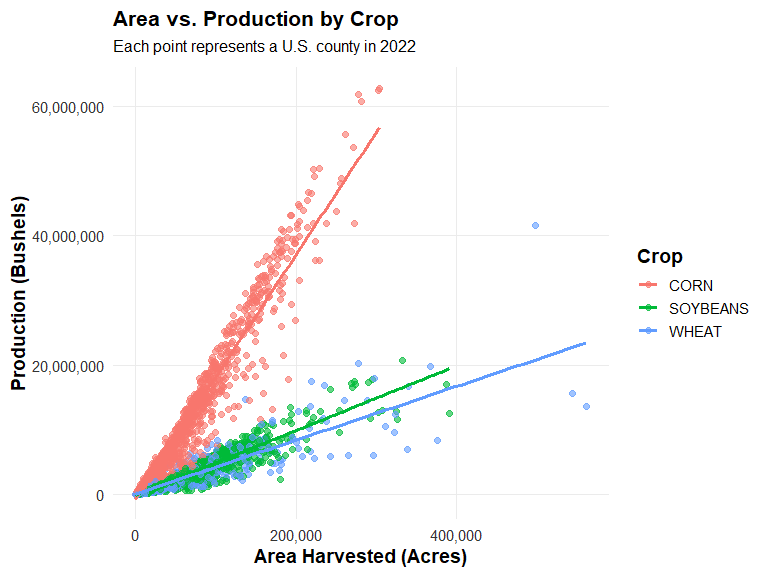
\includegraphics[width=0.9\textwidth]{prod_area.png}
    \caption{Area Harvested vs. Production by Crop. Corn demonstrates the highest production efficiency per acre, while wheat shows lower efficiency.}
\end{figure}

\section{Methods}\label{methods}

As shown in the previous section, there is a clear association between
production, area harvested, and sales. Therefore, we include all three
as predictors in our multiple linear regression model: \[
E[\text{ GDP } | \text{ production, area, sales, crop }] = \beta_0 + \beta_1 \cdot \text{production} + \beta_2 \cdot \text{area} + \beta_3 \cdot \text{sales} + \beta_4 \cdot \text{crop}
\] We also include crop type as a categorical variable to adjust for
structural differences in economic impact across crops, since different
crops vary in both market value and yield characteristics.

Because we are primarily interested in the effect of crop production on
county GDP, we frame the following hypothesis test:

\begin{itemize}
\tightlist
\item
  Null hypothesis \((H_0)\): There is no association between production
  and GDP. \[
  H_0: \beta_1 = 0
  \]
\item
  Alternative hypothesis \((H_A)\): There is an association between
  production and GDP. \[
  H_A: \beta_1 \neq 0
  \] This model allows us to assess whether production contributes
  significantly to explaining variation in GDP, while controlling for
  harvested area, sales, and crop type.
\end{itemize}

\section{Results}\label{results}

After fitting the model, we obtain the following regression
coefficients:

\begin{figure}[H]
    \centering
    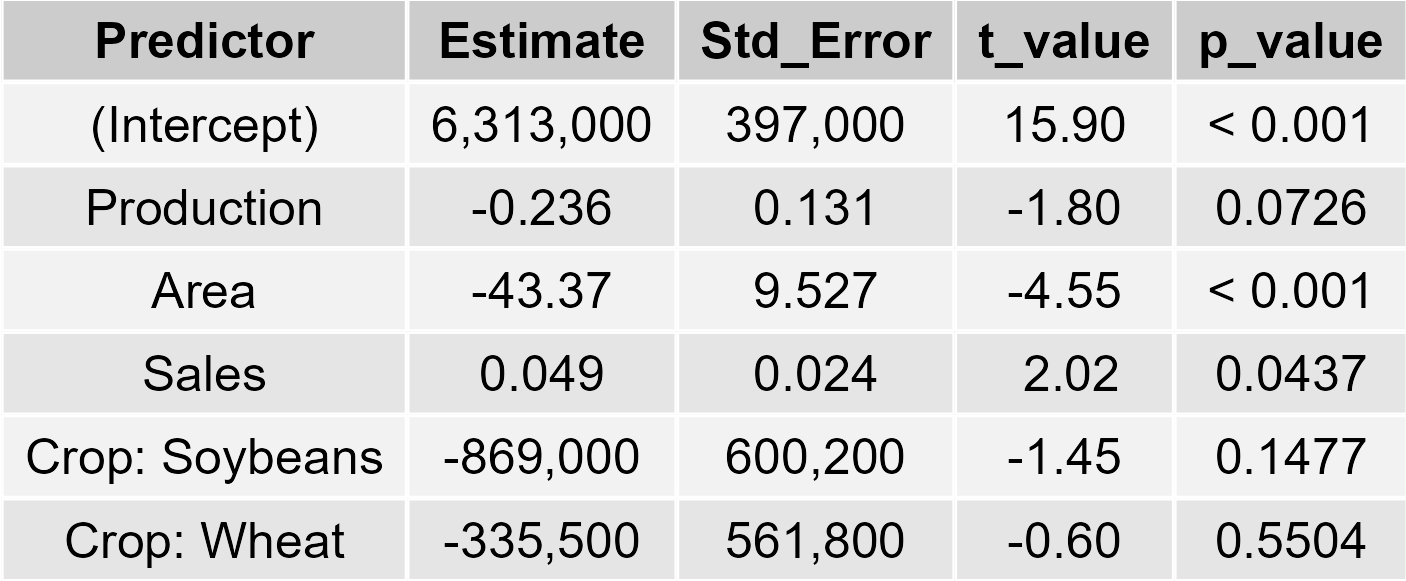
\includegraphics[width=0.6\textwidth]{coef_table.png}
    \caption{Regression coefficients for the model: GDP - Production + Area + Sales + Crop.}
\end{figure}

These results suggest that, holding area, sales, and crop type constant,
an increase of 1 bushel in crop production is associated with an average
decrease of \(\$236\) in GDP. However, this effect is not statistically
significant \((p = 0.0726)\).

In contrast, area harvested is statistically significant
\((p < 0.001)\), indicating a negative association between area and GDP
after adjusting for other variables. Specifically, for each additional
acre harvested, county GDP decreases by an average of \(\$43,370\).

Based on the p-values, we fail to reject the null hypothesis regarding
the effect of production on GDP. However, we find sufficient evidence to
support a negative relationship between harvested area and GDP. It is
plausible that an increase of one acre in harvested area is associated
with a decrease in GDP between \(\$24,316\) and \(\$62,424\).

\section{Conclusion}\label{conclusion}

This study examined whether higher production of major cash crops -
corn, soybeans, and wheat - is associated with higher county-level GDP.
While we found no significant relationship between production and GDP,
we did find a significant negative association between harvested area
and GDP. On average, increasing harvested area by one acre is linked to
a GDP decrease of \(\$24,316\) to \(\$62,424\), after adjusting for
other variables.

This may reflect the fact that agriculture-intensive counties are fewer
and often more rural, while non-agricultural land use may contribute
more to local GDP. It might be economically wise for some counties to
focus less on agriculture, while a smaller number of high-output
counties continue producing enough food for the nation.

Still, agriculture isn't just about GDP. Food is essential to life, and
these crops support broader systems like livestock production. So while
GDP is a useful metric, decisions around agriculture must also consider
food security and sustainability.

This analysis is based on 2022 data and cannot establish causality.
Future studies could include time trends or more detailed measures like
yield or regional effects.

\printbibliography

\end{document}
